\section{Results}
\label{sec:results}
% generated by analysis/analysis.R: provenance of the paper's numbers
\def\EOneMislabeled{1200}
\def\EOneFusedWrong{0}
\def\EOneFusedUp{0.25}
\def\EOneLabel{confirmatory}
\def\EOneRuns{144}
\def\EOneCampaigns{hermes-E1-confirmatory-20261012T053433Z, hermes-E1-confirmatory-20261012T054704Z}
\def\ETwoLabel{confirmatory}
\def\ETwoRuns{120}
\def\EThreeLabel{confirmatory}
\def\EThreeRuns{40}
\def\EOneFastCells{96}
\def\EOneFastEqual{96}
\def\EOneFastRuns{24}
\def\EFourLabel{confirmatory}
\def\EFourRuns{40}
\def\EFourMCP{1.6.0}
\def\EFiveLabel{confirmatory}
\def\EFiveRuns{144}
\def\EFiveConnAuto{8400}
\def\EFiveWrongAuto{0}
\def\ESixLabel{confirmatory}
\def\ESixRuns{96}
\def\ESixDecAuto{6000}
\def\ESevenLabel{confirmatory}
\def\ESevenRuns{26}
\def\ESevenConn{260}
\def\ESevenWrong{0}
\def\ESevenDec{312}
\def\ESevenDecOK{312}
\def\ESevenFA{0}
\def\ESevenFD{0}
\def\ESevenND{0}
\def\ESevenToolMs{9}
\def\EThreeBLabel{confirmatory}
\def\EThreeBRuns{80}
\def\ETwoBLabel{confirmatory}
\def\ETwoBRuns{100}
\def\AgentnetdRuns{594}
\def\AgentnetdEqual{594}
\def\EFiveNetLabel{confirmatory}
\def\EFiveNetRuns{144}
\def\EFiveNetConnAuto{8544}
\def\EFiveNetWrongAuto{0}
\def\EFiveNetCapture{16800}
\def\EFiveNetAttempted{16800}
\def\EFiveNetAsyncManMin{7}
\def\EFiveNetAsyncManMax{30}
\def\EFiveNetMaxDiff{4}
\def\ESixNetLabel{confirmatory}
\def\ESixNetRuns{96}
\def\ESixNetDecAuto{6000}
\def\ESixNetErrAuto{0}
\def\ESevenMLabel{confirmatory}
\def\ESevenMRuns{104}
\def\ESevenMConn{2134}
\def\ESevenMWrong{0}
\def\ESevenMAmb{0}
\def\ESevenMDec{1872}
\def\ESevenMDecOK{1872}
\def\ESevenMFA{0}
\def\ESevenMFD{0}
\def\ESevenMND{0}
\def\ESevenMToolMs{10}
\def\ESevenCLabel{confirmatory}
\def\ESevenCRuns{104}
\def\ESevenCConn{1560}
\def\ESevenCWrong{0}
\def\ESevenCAmb{0}
\def\ESevenCDec{1872}
\def\ESevenCDecOK{1872}
\def\ESevenCUSD{4.60}
\def\ESevenCInTok{1952}
\def\ESevenCOutTok{280}
\def\ESevenOLabel{confirmatory}
\def\ESevenORuns{104}
\def\ESevenOConn{1560}
\def\ESevenOWrong{0}
\def\ESevenOAmb{0}
\def\ESevenODec{1872}
\def\ESevenODecOK{1872}
\def\ESevenOUSD{0.86}
\def\ESevenOInTok{730}
\def\ESevenOOutTok{117}
\def\ESevenOReasTok{1}
\def\ESevenRRuns{416}
\def\ESevenRSame{416}
\def\ESevenRCalls{416}
\def\ESevenRConn{6240}
\def\ESevenRWrong{0}
\def\ESevenRDec{7488}
\def\ESevenRDecOK{7488}
\def\EThreeNetLabel{confirmatory}
\def\EThreeNetRuns{40}
\def\EThreeNetBase{59}
\def\EThreeNetAdd{12.2}
\def\EThreeNetAddMk{20.2}
\def\EThreeNetRel{21}
\def\APRuns{72}
\def\APConn{8400}
\def\APWrongMin{92}
\def\APWrongMax{96}
\def\APWrongTwoMin{54}
\def\APWrongTwoMax{92}
\def\APSubMin{7}
\def\APSubMax{58}
\def\APAgentnetWrong{0}
\def\APAgentnetConn{8400}
\def\ResultsBanner{}

\IfFileExists{generated/baselines_meta.tex}{% generated by analysis/baselines_table.py
\def\BaseRuns{60}
\def\BaseCampaigns{hermes-E1-confirmatory-20261012T053433Z, hermes-E1-confirmatory-20261012T054704Z, hermes-E5-confirmatory-20261012T181111Z, hermes-E5-confirmatory-20261012T195813Z}
\def\BaseNearErrEveryRun{yes}
\def\BaseOursWrong{0}
}{\def\BaseRuns{\TBD}}
\IfFileExists{generated/fault_meta.tex}{% generated by analysis/fault_tables.py
\def\FaultEsevenMis{104}
\def\FaultEsevenFA{0}
\def\FaultEsevenAllowed{0}
\def\FaultEsevenFD{86}
\def\FaultEsevenRuns{26}
\def\FaultEsevenOther{0}
\def\FaultEfiveRuns{128}
\def\FaultEsixRuns{128}
\def\FaultConn{16000}
\def\FaultMis{1920}
\def\FaultMisWrong{1920}
\def\FaultSpill{0}
\def\FaultPolMis{1920}
\def\FaultPolErr{1112}
\def\FaultPolErrPct{58}
\def\LinRuns{96}
\def\LinConflictsExact{yes}
\def\LinModeTwoErr{0}
\def\LinModeTwoDec{6400}
\def\LinModeOneFA{0}
\def\LinModeZeroErr{592}
\def\LinModeZeroMis{800}
\def\LinModeZeroPct{74}
\def\LsRuns{48}
\def\LsDecisions{6000}
\def\LsErrors{0}
\def\LsConflicts{0}
\def\FaultCampaigns{hermes-E5f-confirmatory-20261013T024326Z, hermes-E5f-confirmatory-20261013T033751Z, hermes-E6L-confirmatory-20261013T023556Z, hermes-E6L-confirmatory-20261013T033021Z, hermes-E6Ls-confirmatory-20261013T023941Z, hermes-E6Ls-confirmatory-20261013T033406Z, hermes-E6f-confirmatory-20261013T025310Z, hermes-E6f-confirmatory-20261013T034734Z, hermes-E7f-confirmatory-20261013T030309Z, hermes-E7f-confirmatory-20261013T035733Z}
}{}
\ResultsBanner

Each subsection opens with its conclusion; unless stated otherwise, numbers come from confirmatory campaigns over two boots.

\subsection{Signal Sufficiency and Fusion}

With correct context, the fused resolver attributes all connections in all four structures; with faulty context, it converts errors into reported ambiguity wherever the process structure can contradict the label (\cf Figure~\ref{fig:e1}). A shared cgroup cannot tell executions apart in N1--N3, nor can lineage in N2--N3, so the single-signal resolvers report ambiguity there. The collector captured all planned connections in all runs.

\begin{figure}[!ht]
\centering
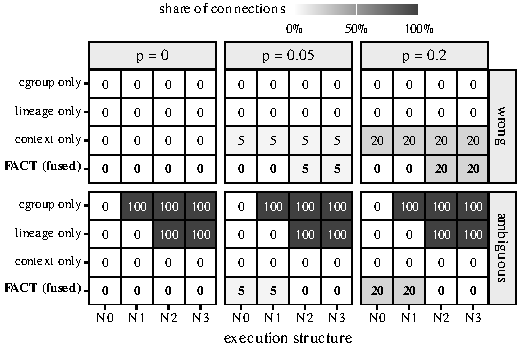
\includegraphics[width=\columnwidth]{generated/fig_e1.pdf}
\caption{E1: percentage of connections credited to the wrong execution (top) or reported as ambiguous (bottom), per resolver, execution structure, and fault fraction $p$ (\EOneRuns\ runs; label: \EOneLabel). Operation modes are pooled; they produced identical counts in every cell.}
\label{fig:e1}
\end{figure}

With correct markers, context-only and fused attribution are correct everywhere, so threads and forked subprocesses inherit the context; mislabeled markers separate them. In N0 and N1, lineage contradicts the label, so the fused resolver flags each mislabeled connection as ambiguous (I/N = 0), whereas context-only credits all of them to the wrong execution. In N2 and N3, both resolvers follow the label, because inside a shared worker no kernel signal can contradict it. The outcome was identical in all \EOneRuns\ confirmatory runs over two boots.

\subsection{Accounting}
The net accounting error hides misattributions, and the decomposition exposes them (Fig.~\ref{fig:acct}). With symmetric mislabels, context-only accounting reports a net error of zero even when a fifth of its connections go to the wrong execution. In N0 and N1, fused accounting moves the mislabeled connections from \emph{wrong} to \emph{uncredited}. Its net error is larger, but it is conservative: across \EOneRuns\ runs, none of the \EOneMislabeled\ mislabeled connections was credited to the wrong execution.

\begin{figure}[!ht]
\centering
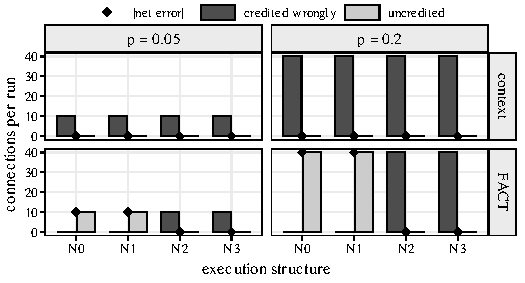
\includegraphics[width=\columnwidth]{generated/fig_acct.pdf}
\caption{E1 accounting with mislabeled markers: connections per run (of 200) credited to the wrong execution or left uncredited, and the absolute net error summed over executions; the remaining connections are credited correctly.}
\label{fig:acct}
\end{figure}

\subsection{Scale and Overhead}

Attribution stays correct and complete up to 64 concurrent executions (E2), and the collector adds microseconds per connection. With $P$ concurrent instances of the closed-loop \texttt{connect} microbenchmark (E2b), capture is complete up to $P{=}4$ (over $10^5$ connections per second); from $P{=}6$ on, with the vCPUs saturated, bpftrace reports lost events, so loss is never silent.

E3 isolates the cost on a closed loop of loopback connections, the worst case for per-connection instrumentation: the collector adds about 8\,$\mu$s to the median \texttt{connect}, and the markers add two failed system calls per operation, costlier when the collector also traces \texttt{openat}. Over the virtual network interface (E3net, \EThreeNetRuns\ runs), the median \texttt{connect} takes \EThreeNetBase\,$\mu$s and the collector adds \EThreeNetAdd\,$\mu$s (\EThreeNetRel\%).

E3b separates the components: attaching the probes while only counting events adds 1.5\,$\mu$s, and exporting one record per connection accounts for most of the remaining 6.7\,$\mu$s, in both the full and the optimized collector. With markers, the optimized variant lowers the added median latency from 19.1 to 14.3\,$\mu$s and the eBPF time per program run from 1304 to 854\,ns. It is a drop-in replacement: rerunning E1 with it (\EOneFastRuns\ runs) reproduced the outcome fractions of the full collector in \EOneFastEqual\ of \EOneFastCells\ cell--resolver combinations.

\subsection{Shared MCP Server}
Thread-keyed context breaks for asynchronous tools; binding the identity to the task fixes it without changing tool code. E4 runs a real MCP server, one process in one cgroup serving $K$ concurrent sessions, so lineage and cgroup are ambiguous for every connection. Synchronous, threaded, and subprocess tools inherit the marker and are attributed correctly; asynchronous tools are not: coroutines of different sessions interleave on the event-loop thread and overwrite its context, so 42\% ($K$=2) and 39\% ($K$=4) of the connections are credited to the wrong session, and connections opened after another coroutine's end marker are ambiguous.

\begin{figure}[t]
\centering
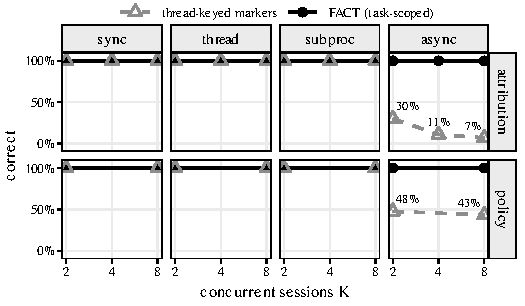
\includegraphics[width=\columnwidth]{generated/fig_e5e6.pdf}
\caption{E5 and E6: correct attribution (top) and correct egress-policy decisions (bottom) in a shared MCP server, per tool type and number of concurrent sessions $K$, with thread-keyed markers (manual) and with the task-scoped binding of \solution{} (fused resolver; \EFiveRuns\ E5 and \ESixRuns\ E6 runs).}
\label{fig:e5e6}
\end{figure}

Figure~\ref{fig:e5e6} (top) compares the two bindings on the same server, tools, and seeds. With manual markers, correct attribution of asynchronous tools falls from 30\% to 7\% as sessions grow, and about 40\% of the connections go to the wrong session at every $K$. With the task-scoped binding, the same tools, without markers, had \EFiveWrongAuto\ errors in \EFiveConnAuto\ connections (a one-sided 95\% Clopper--Pearson bound of 0.2\% at $K{=}8$). Both bindings are correct for the other tools, with median tool-call latencies within 0.2\,ms. Across a real network interface the outcome is the same (E5net and E6net, \EFiveNetRuns\ and \ESixNetRuns\ runs): manual markers fall from \EFiveNetAsyncManMax\% to \EFiveNetAsyncManMin\% correct for asynchronous tools, and the task-scoped binding made \EFiveNetWrongAuto\ errors in \EFiveNetConnAuto\ connections (144 of them identity-less reachability probes, reported as unattributed) and \ESixNetErrAuto\ policy errors in \ESixNetDecAuto\ decisions.

\begin{figure}[t]
\centering
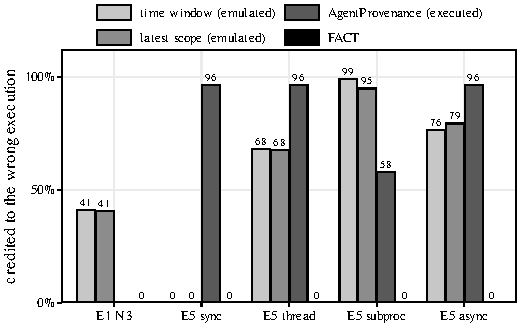
\includegraphics[width=\columnwidth]{generated/fig_baselines.pdf}
\caption{Related systems vs.\ \solution{} in shared workers (E1 N3, $p=0$; E5, $K=8$): percentage of connections credited to the wrong execution. Emulations (\BaseRuns\ runs) use the manual-mode call boundaries; AgentProvenance was executed in the E5 rounds (E5ap).}
\label{fig:base}
\end{figure}

\subsection{Comparison with Related Mechanisms}
Time-based and latest-binding correlation cannot separate concurrent tool calls inside one process; \solution{} can. We emulate the documented mechanisms of related systems as offline resolvers over the same logs, with process lineage first and the tool-call boundaries of the manual mode (Fig.~\ref{fig:base}): the \emph{time-window} resolver picks the latest tool-call start within 500\,ms, as in AgentSight, and the \emph{latest-scope} resolver picks the open binding that started last, as in AgentProvenance. With distinct process trees (N0, N1), lineage alone suffices. Inside a shared worker, time separates only blocking calls: both misattribute 41\% of the connections in N3 and 68--99\% for threaded, subprocess, and asynchronous tools with eight sessions.

Running AgentProvenance itself confirms the mechanism and shows the emulation was optimistic (E5ap, \APRuns\ runs). With four and eight sessions it credited \APWrongMin--\APWrongMax\% of the connections of synchronous, threaded, and asynchronous tools to the wrong session (\APWrongTwoMin--\APWrongTwoMax\% with two), and \APSubMin--\APSubMax\% for subprocess tools, whose child processes it can sometimes match; \solution{} misattributed \APAgentnetWrong\ of \APAgentnetConn\ connections in the same rounds. Its harness sees each call's window from the client, so when a tool connects all $K$ windows are open and it picks the latest. AgentSight attributes per process, so in a shared server it cannot name a session; we keep it emulated.

\subsection{Egress Policy and LLM Agents}
Binding errors turn into policy errors in both directions, and the task-scoped binding removes them. With manual markers and asynchronous tools, only 48\% ($K$=2) and 43\% ($K$=8) of the decisions are correct (Fig.~\ref{fig:e5e6}, bottom): mislabeled restricted executions pass (9--11\% false allows, \ie bypasses) and others are blocked (42--48\% false denies). With the task-scoped binding, all \ESixDecAuto\ decisions match the reference. Connections without identity are denied by default, so a missing binding fails closed instead of inheriting a guess.

In E7 the tool calls are chosen by a language model. Four agents share one MCP server process in one cgroup; the fused resolver attributed \ESevenWrong\ of \ESevenConn\ connections incorrectly, and the policy made \ESevenDecOK\ correct decisions out of \ESevenDec. The median tool call took \ESevenToolMs\,ms, against several seconds per model step. With larger models on a GPU and up to eight agents (E7m, \ESevenMRuns\ runs), the result is the same: \ESevenMWrong\ of \ESevenMConn\ connections were misattributed, and \ESevenMDecOK\ of \ESevenMDec\ policy decisions were correct. Commercial models from Anthropic and OpenAI agree (\ESevenCRuns\ runs each): with Claude (E7c), \ESevenCWrong\ of \ESevenCConn\ connections misattributed and \ESevenCDecOK\ of \ESevenCDec\ decisions correct; with GPT (E7o), \ESevenOWrong\ of \ESevenOConn\ and \ESevenODecOK\ of \ESevenODec, for US\$\,\ESevenCUSD\ and US\$\,\ESevenOUSD\ in API tokens. Replayed without the models (E7r), \ESevenRSame\ of \ESevenRRuns\ runs reproduced the same calls and outcomes, so the results do not depend on the models staying available.

\begin{table}[t]
\centering
\caption{Binding faults injected into the framework: a fraction $p$ of each execution's tool calls carries another execution's identity (task-scoped binding; tools pooled; \FaultEfiveRuns\ E5f, \FaultEsixRuns\ E6f, and \FaultEsevenRuns\ E7f runs). Wrong: mislabeled connections credited to the wrong execution; other err.: errors on correctly labeled calls.}
\label{tab:fault}
\footnotesize
\setlength{\tabcolsep}{2.2pt}
\IfFileExists{generated/tab_fault.tex}{% gerado por analysis/fault_tables.py — não editar à mão
\begin{tabular}{@{}lrrrrrrr@{}}
\toprule
 & & \multicolumn{3}{c}{attribution (E5f)} & \multicolumn{3}{c}{policy (E6f, E7f)} \\
\cmidrule(lr){3-5}\cmidrule(l){6-8}
$K$ & $p$ & mislab. & wrong & other err. & FA & FD & other err. \\
\midrule
2 & 0.04 & 64 & 64 & 0 & 16 & 32 & 0 \\
2 & 0.20 & 320 & 320 & 0 & 80 & 160 & 0 \\
8 & 0.04 & 256 & 256 & 0 & 72 & 64 & 0 \\
8 & 0.20 & 1280 & 1280 & 0 & 208 & 480 & 0 \\
\midrule
\multicolumn{2}{l}{E7f (LLM)} & 104 & 0 & 0 & 0 & 86 & 0 \\
\bottomrule
\end{tabular}
}{\TBD}
\end{table}

\begin{table}[t]
\centering
\caption{E6L: policy decisions with mislabeled calls when executions have their own process trees (N0 and N1, both operation modes pooled; \LinRuns\ confirmatory runs over two boots). Conflicts: contradictions between label and process tree flagged in the kernel.}
\label{tab:lineage}
\footnotesize
\setlength{\tabcolsep}{2.4pt}
\IfFileExists{generated/tab_lineage.tex}{% generated by analysis/fault_tables.py; do not edit by hand
\begin{tabular*}{\columnwidth}{@{\extracolsep{\fill}}lrrrrrr@{}}
\toprule
Lineage check & $p$ & decisions & mislab. & conflicts & FA & FD \\
\midrule
label only & 0.05 & 3200 & 160 & -- & 48 & 80 \\
label only & 0.20 & 3200 & 640 & -- & 144 & 320 \\
deny on conflict & 0.05 & 3200 & 160 & 160 & 0 & 112 \\
deny on conflict & 0.20 & 3200 & 640 & 640 & 0 & 496 \\
tree owner & 0.05 & 3200 & 160 & 160 & 0 & 0 \\
tree owner & 0.20 & 3200 & 640 & 640 & 0 & 0 \\
\bottomrule
\end{tabular*}
}{\TBD}
\end{table}

\subsection{Faulty Bindings}

A faulty label affects only its own call, and wherever executions have their own process trees, the in-kernel lineage check stops the bypasses it would cause. In the shared MCP server (Table~\ref{tab:fault}), every mislabeled connection is credited to the execution named by the label (\FaultMisWrong\ of \FaultMis), and no other connection or decision is affected (\FaultSpill\ errors elsewhere): because the identity is bound to the task, a faulty call does not contaminate later calls. No kernel signal contradicts a label inside one process, so \FaultPolErrPct\% of the mislabeled calls also became policy errors, in both directions. The LLM agents have disjoint allow-lists, so \FaultEsevenAllowed\ of their \FaultEsevenMis\ mislabeled calls were allowed: the fault failed closed. Where executions have their own process trees, the lineage check moves the offline detection of contradicted labels (E1) into the kernel (Table~\ref{tab:lineage}). With the label alone, the policy decided \LinModeZeroPct\% of the mislabeled connections wrongly. Denying on conflict removed every false allow, and deciding by the tree owner removed every decision error (\LinModeTwoErr\ in \LinModeTwoDec\ decisions); in both modes, the conflicts flagged in the kernel were exactly the mislabeled connections. In the shared server, where the tree is shared and therefore not registered, the check vetoed none of \LsDecisions\ correct decisions (E6Ls).

Finally, \texttt{factd}, fed the recorded collector streams in arrival order with a 100\,ms reordering window, reproduced the per-execution credited, ambiguous, and unattributed counts of the offline evaluation in \AgentnetdEqual\ of \AgentnetdRuns\ runs.
